\subsubsection{Comparacion de Kruskal contra Prim}

Al comparar Prim y Kruskal a la hora de clusterizar, podemos ver que ambos producen resultados similares. La diferencia entre ambos existe a la hora de generar el árbol generador mínimo, sobre el cual luego se descartan los ejes inconsistentes.

\begin{figure}[H]
	\centering
	\begin{minipage}[t]{.3\textwidth}
		\centering
		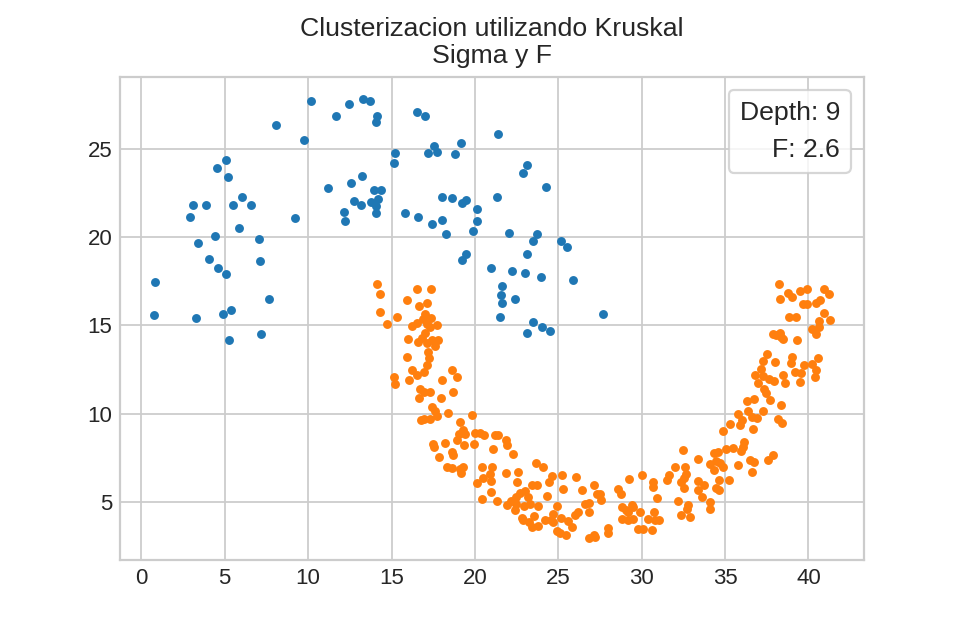
\includegraphics[scale=0.4]{experimentos/kvp-dataset-11-Kruskal}
	\end{minipage}\qquad
	\begin{minipage}[t]{.3\textwidth}
		\centering
		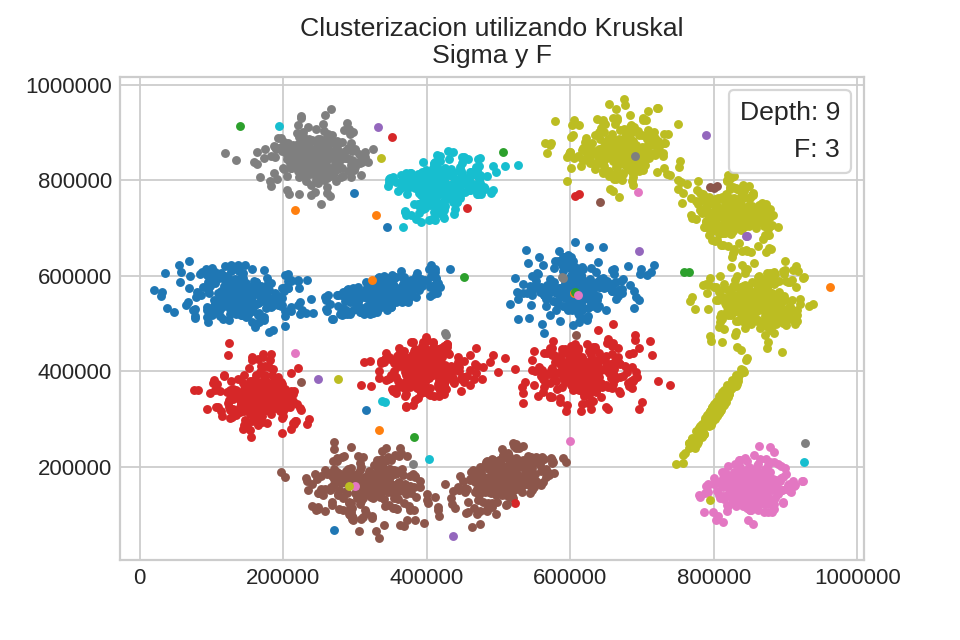
\includegraphics[scale=0.4]{experimentos/kvp-dataset-4-Kruskal}
	\end{minipage}\qquad
	\begin{minipage}[t]{.3\textwidth}
		\centering
		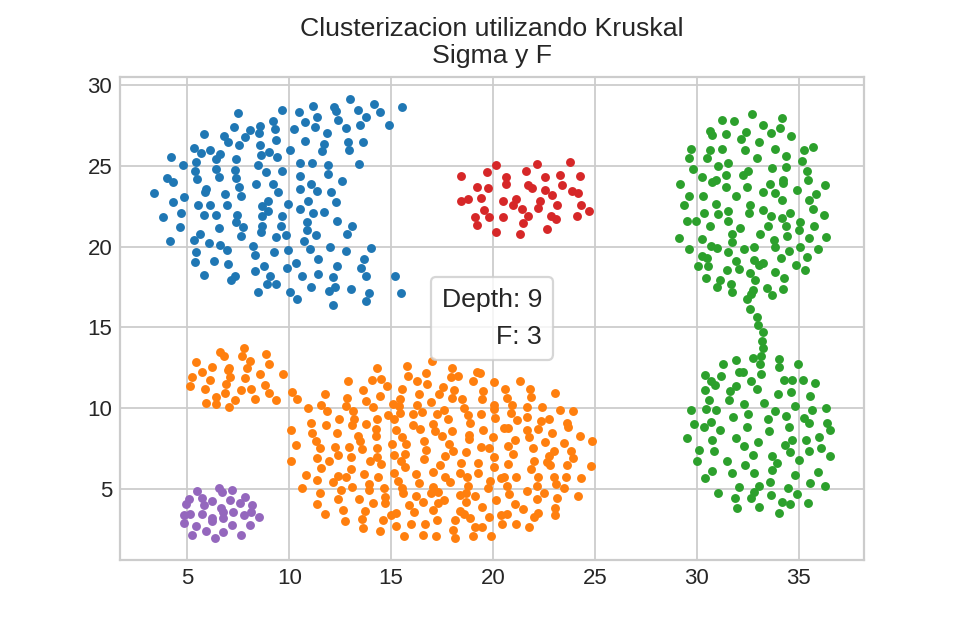
\includegraphics[scale=0.4]{experimentos/kvp-dataset-6-Kruskal}
	\end{minipage}
\end{figure}	

\begin{figure}[H]
	\centering
	\begin{minipage}[t]{.3\textwidth}
		\centering
		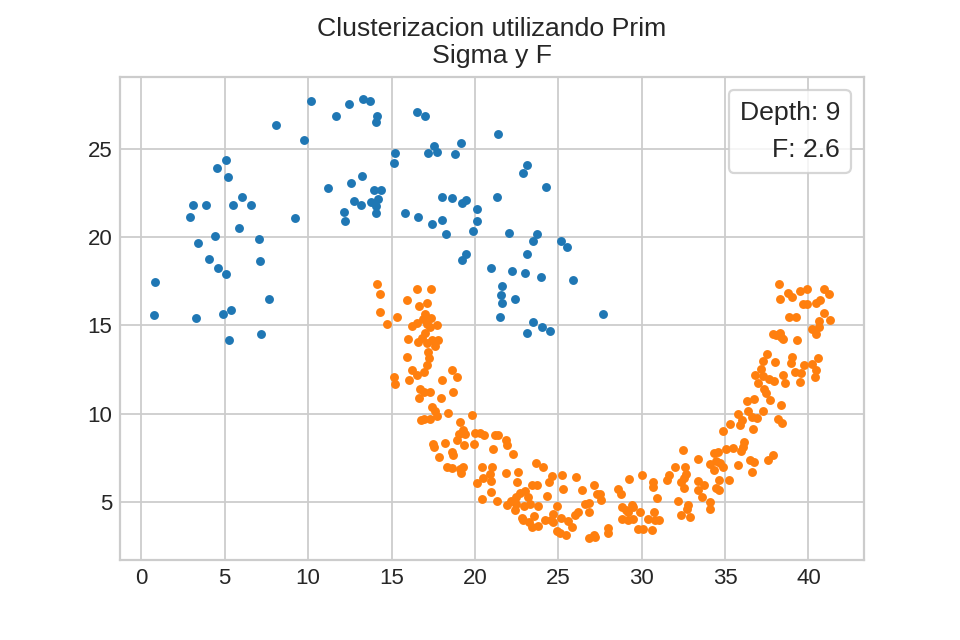
\includegraphics[scale=0.4]{experimentos/kvp-dataset-11-Prim}
	\end{minipage}\qquad
	\begin{minipage}[t]{.3\textwidth}
		\centering
		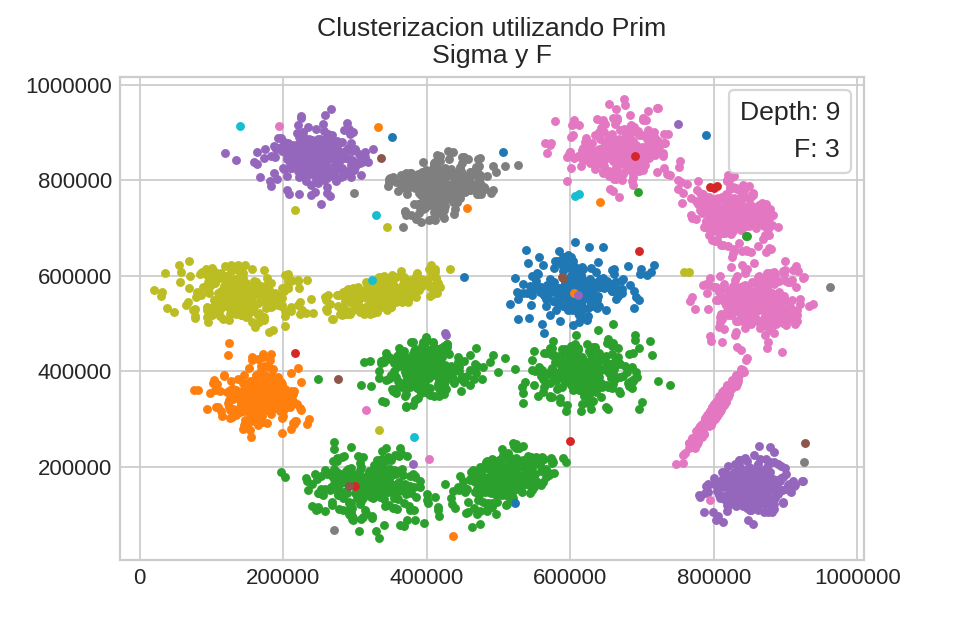
\includegraphics[scale=0.4]{experimentos/kvp-dataset-4-Prim}
	\end{minipage}\qquad
	\begin{minipage}[t]{.3\textwidth}
		\centering
		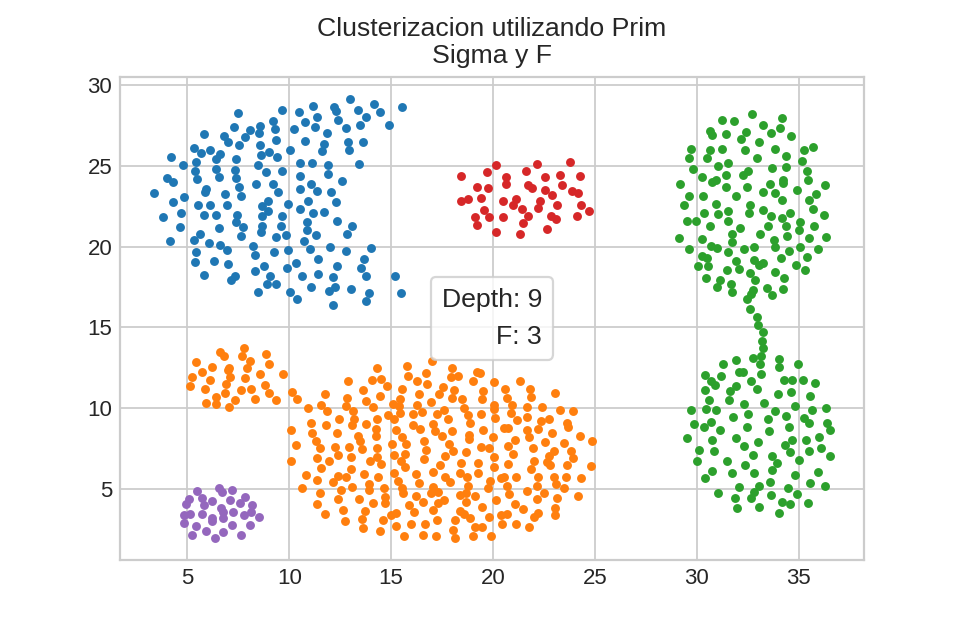
\includegraphics[scale=0.4]{experimentos/kvp-dataset-6-Prim}
	\end{minipage}
\end{figure}	

\subsubsubsection{Conclusiones}

Sin embargo, cabe destacar para Kruskal -al ser un algoritmo bottom up- armar los clusters una vez recortado el árbol generador mínimo es una tarea trivial, ya que el algoritmo se basa en formar clusters desconectados. En este aspecto, debemos realizar una solución Ad-Hoc para Prim, lo cual nos fuerza a obtener una complejidad mayor, a fuerza de no implementar Kruskal para clusterizar dentro de Prim.

\begin{figure}[H]
	\centering
	\begin{minipage}[t]{.45\textwidth}
		\centering
		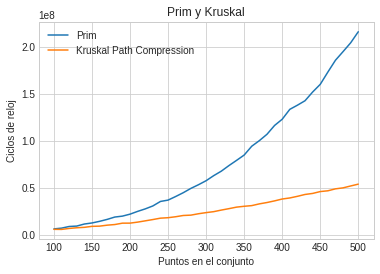
\includegraphics[scale=0.55]{experimentos/prim-v-kruskal}
	\end{minipage}\qquad
	\begin{minipage}[t]{.45\textwidth}
		\centering
		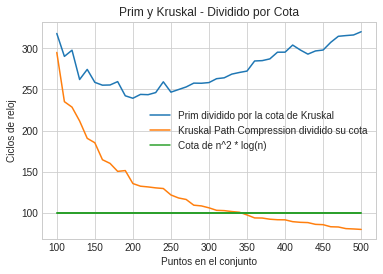
\includegraphics[scale=0.55]{experimentos/prim-v-kruskal-acotado}
	\end{minipage}
\end{figure}	
